%%==================================================
%% chapter02.tex for SJTU Master Thesis
%% based on CASthesis
%% modified by wei.jianwen@gmail.com
%% Encoding: UTF-8
%%==================================================

\chapter{流体模拟的基本方法与框架}
\label{chap:fluidSimulation}

\section{Navier-Stokes方程组}
\label{sec:navier-stokes}

计算机图形学最有趣的问题之一是类流体行为的仿真,不同领域的对流体模拟求解的目标由不同的要求。在特效产业中,令人信服地模仿譬如烟雾、水和火等流体的外观和行为,是极其需要的;在计算机动画领域,模拟流体动画,我们更关心的是视觉效果,而不是求解的准确性,特别地,对烟而言,我们更关心烟动画中的小规模细节,而不是速度场的数值精度。在基于仿真上,流体力学被作为标准数学框架在使用。科学家们一致表示,Navier-Stokes方程式是流体流动的一个很好的数学模型。

\subsection{Navier-Stokes方程组的描述形式}

在流体力学中,Navier-Stokes方程组描述了不可压的粘性牛顿流体的方程,被称为世界上“最复杂的方程之一”。Navier-Stokes方程组的名字记录了导出该方程组的人的姓名,分别是Claude Louis Navier 和 George Gabriel Stokes,通常也可简称为N-S方程组。通常可以写成如下形式~\cite{bridson2007fluid}:

\begin{equation}
\label{basicEq}
 \frac{\partial \boldsymbol u}{\partial t} + {\boldsymbol u} \cdot \nabla {\boldsymbol u} + \frac{1}{\rho} \nabla p= {\boldsymbol g} + \upsilon \nabla \cdot \nabla {\boldsymbol u}
\end{equation}

\begin{equation}
\label{imcompressible}
 \nabla \cdot {\boldsymbol u} = 0
\end{equation}
 
\(\boldsymbol u\)表示流体的速度场。在欧拉方法中,该速度表示流体经过每个固定的点空间时所具有的速度矢量。在3D情况下,\(\boldsymbol u\)通常表示成\((u,v,w)\)的形式,分别表示3D空间标准坐标系下的\(\boldsymbol{x}, \boldsymbol{y}, \boldsymbol{z}\)三个方向上的速度大小。
 
\(p\) 表示压强场,在流体的内部,每个欧拉网格的内部都有一个压强分量。

\(t\)代表时间。
 
\(\upsilon\)代表流体的粘性系数,\(\upsilon\)越大,表示流体的粘性越大。
 
\(\rho\)表示流体的密度。
  
 \(\boldsymbol g\)表示施加在流体上的外力合力产生的加速度,这些外力包括重力、浮力等。大部分情况下,流体只受重力的影响,故在此用了通常表示重力加速度的\(\boldsymbol g\)表示。
 
 \(\nabla\)是向量空间的偏导数, 如\(\nabla {\boldsymbol u}\)表示速度场的偏导数。\(\nabla\) = (\(\frac{\partial}{\partial x}, \frac{\partial}{\partial y})\)表示2D空间的偏导,\(\nabla\) = (\(\frac{\partial}{\partial x}, \frac{\partial}{\partial y}, \frac{\partial}{\partial z})\) 则表示3D空间的偏导。另外,\(\nabla \cdot \nabla\)表示拉普拉斯算子。

\subsection{Navier-Stokes方程组的意义}
\label{sec:eqmeaning}
Navier-Stokes方程组对流体做了以下几个假设:第一,流是连续的。该假设强调液体内部不包含空隙,如溶解的气体的气泡,而且它不包含雾状粒子的聚合。第二,所有涉及到的场都是可微的,如压强场、速度场、密度和温度等。

Nacier-Stokes方程组的式~\ref{basicEq}根据质量,动量,和能量的守恒的基本原理导出。我们可以把流体模拟想象成一个粒子系统,每个粒子代表一个小水珠。那么,我们可以描述每个粒子的质量为\(m\),速度为\(\boldsymbol u\),体积为\(V\)。那么根据动量守恒定理,我们可以得到如下方程式:

\begin{equation}
\label{momentum}
 {\boldsymbol F} = m\frac{D{\boldsymbol u}}{D{t}}
\end{equation}

假设粒子受到的来自流体系统以外的力只有重力,表示为\(m{\boldsymbol g}\)。那么我们只需要分析流体粒子来自于粒子系统中其他粒子的力。

首先是压力。流体在运动的过程中,压力的作用会把高压区的流体推向低压区,从而使得流体粒子在整体上始终保持均匀分布得趋势。图\ref{pressuredepth}画出了流场内部流体粒子所有压力的示意图。从左边的图中,我们可以看出流体粒子所受的压力来自四面八方。我们假设粒子每个方向上所受的压力都相等,根据图\ref{pressuredepth}右边的示例图片,可知流体粒子的压力只与其深度有关。为了简化模型,我们用压强梯度的负值\(-\nabla p\)表示压强的不平衡效果,而\(({-\nabla p})V\)表示粒子所有到的压力。

然后是粘滞力。粘滞力总是阻碍两个粒子之间的相对运动,并且相对运动越大,粘滞力越大。这里,我们直接给出粘滞力的表达式为\(V\mu{\nabla \cdot \nabla {\boldsymbol u}}\)。其中,\(\mu\)为动态粘性系数,是流体自身的属性,通常是常量。故用重力、压力以及粘滞力表示方程式~\ref{momentum}中的外力\(\boldsymbol F\),可得到流体运动的加速度方程:

\begin{equation}
 m\frac{D{\boldsymbol u}}{D{t}} = m{\boldsymbol g} - V{\nabla p} + V{\mu}{\nabla \cdot \nabla {\boldsymbol u}}
\end{equation}

\begin{figure}
  \centering
   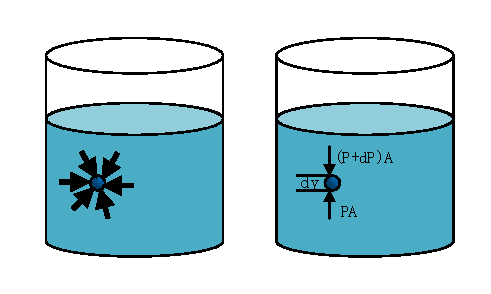
\includegraphics[height=1.8 in]{chap2/pressuredepth}
  \bicaption[pressuredepth]{}{流体粒子受压力示意图}{Fig}{Illustration of how fluid particles are affected by pressure}
\end{figure}

我们已知\(\frac{V}{m} = \frac{1}{\rho}\),设变量\(\upsilon = \frac{\mu}{\rho}\),上述方程式两边都除以粒子的质量m,则有:

展开速度场\(\boldsymbol u\)关于时间\(t\)的导数,即可得到方程式~\ref{basicEq}。

\begin{figure}
  \centering
   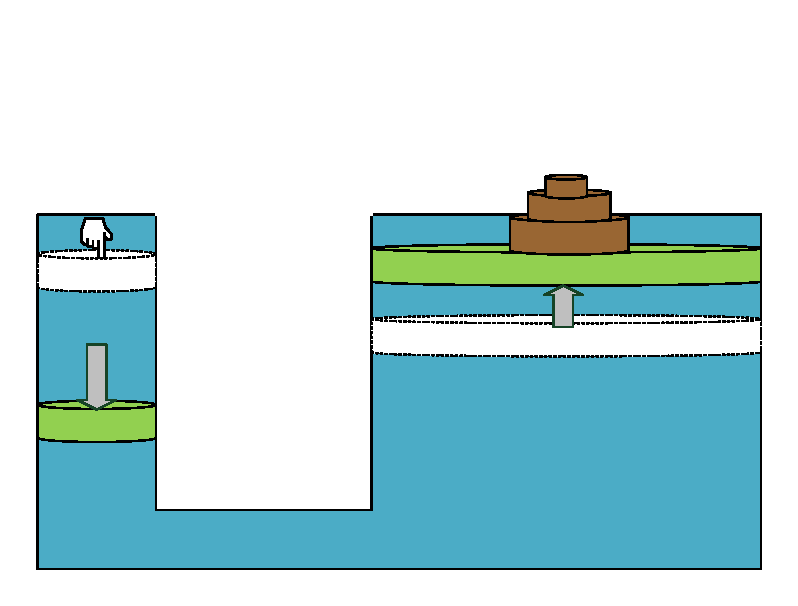
\includegraphics[height=2.3 in]{chap2/imcompressible}
  \bicaption[fig:imcompressible]{}{流体不可压示意图}{Fig}{Illustration of imcompressible condition}
\end{figure}

方程式~\ref{imcompressible}表示流体的不可压缩条件。图~\ref{fig:imcompressible}展示了流体不可压缩时的宏观表现,即压缩流体时,流体会保持其体积不变。从微观的角度讲,当我们说流体是不可压缩的时,指的是在微观时间段\(\delta t\)内,流入与流出流体任意体积为\(\Omega\)的流体表面的体积是相等的,即流体的体积变化速率为0,可以表示成如下形式:

\begin{equation}
{\iint_{\partial \Omega}}{\boldsymbol u} \cdot {\hat n} = 0 
\end{equation}

根据微积分基本定理,我们可以将上式转化为如下形式:

\begin{equation}
{\iiint_{\Omega}} \nabla \cdot {\boldsymbol u} = 0 
\end{equation}

由于上述方程式对于流体内部的任意体积\(\Omega\)都是成立的,故只有当被积函数处处为0时,上述函数积分才能为0。即为方程式~\ref{imcompressible}。

\subsection{忽略粘性力作用}

通常,在计算机动画模拟的数值计算中,会忽略掉粘性力这一项。因为相比较于其他作用力,粘性力的值通常是很小的。另外,在流体模拟的数值计算的过程中不可避免地会有数值耗散,而该数值耗散项的值的数量级与粘性力项的值的数量级比较接近,故可以近似认为数值耗散项替代了粘性力项的计算。并且从方程式~\ref{basicEq}中,我们可以看出,粘性力项的计算开销也比较大。故流体模拟的一般方法求解的是如下形式的Navier-Stokes方程组:

\begin{equation}
\label{basicEqignoreVis}
 \frac{\partial \boldsymbol u}{\partial t} + {\boldsymbol u} \cdot \nabla {\boldsymbol u} + \frac{1}{\rho} \nabla p= {\boldsymbol g}
\end{equation}

\section{流体模拟的基本方法与框架}

根据绪论部分的介绍,我们可知目前现有的流体模拟方法主要有三大类,即欧拉网格法、拉格朗日粒子法和基于旋度的方法。本文主要研究基于欧拉网格方法的重构上采样框架,故本章的该部分将会重点介绍用欧拉网格法求解Navier-Stokes方程组的框架。

\subsection{网格介绍}

\begin{figure}
  \centering
   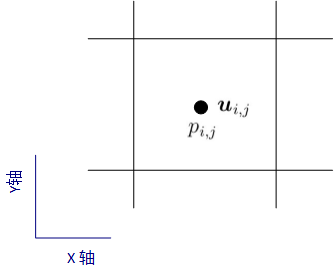
\includegraphics[height=1.6 in]{chap2/centergrid2D}
  \bicaption[fig:centergrid2d]{}{中心网格2D示意图}{Fig}{cells from 2D center grid}
\end{figure}

用欧拉方法求解流体动画时,需要在网格上对其进行求解计算。最简单的网格模型是中心网格,该网格模型把所有的变量都存储在网格的中心点上,如图~\ref{fig:centergrid2d}描述了中心网格在2D场景下变量的存储方式。但是被更加广为使用的是MAC网格模型,由Harlow等人~\cite{harlow1965numerical}提出。MAC网格实际上时一个交错的网格,变量存储在网格的不同位置上,并且存储在不同位置的变量有不同的含义,如图~\ref{fig:macgrid}所示,(a)和(b)分别描述了2D场景和3D场景下MAC网格各变量的存储方式,其中\(p\)是压力值,\(u,v,w\)分别表示速度场的三个分量。相较于中心网格,MAC网格的计算效率更高,并且更加稳定。本文提出的流体模拟重构框架既适用于中心网格,也适用于MAC网格。

\begin{figure}
  \centering
   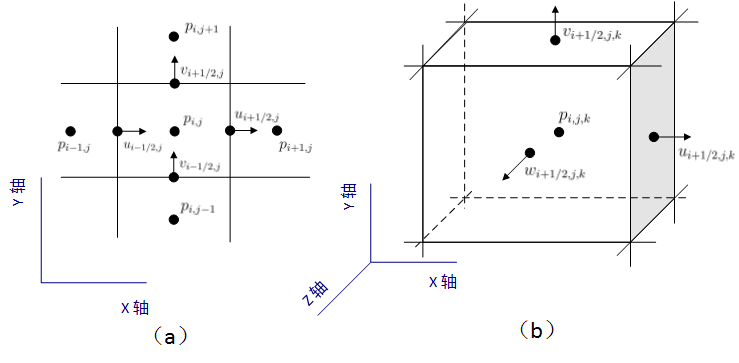
\includegraphics[height=2.5 in]{chap2/macgrid}
  \bicaption[fig:macgrid]{}{(a) 2D MAC网格示意图;(b) 3D MAC网格示意图}{Fig}{(a) one cell from the 2D MAC grid;(b) one cell from the 3D MAC grid}
\end{figure}

\subsection{欧拉方法的基本框架}

Navier-Stokes方程组方程组虽然看起来简单,但是因为方程式~\ref{basicEqignoreVis}存在非线性项,故直接求解非常困难。为了简化求解过程,通常会把Navier-Stokes方程组分解成三个部分求解,分别为对流、体积力和压力/不可压缩部分。分别列出如下:

\begin{equation}
\label{eq:advection}
\frac{\partial {\boldsymbol u}}{\partial t} + {\boldsymbol u} \cdot \nabla {\boldsymbol u} = 0  \ \ \ \ \ (advection)
\end{equation}
\begin{equation}
\label{eq:addForce}
\frac{\partial {\boldsymbol u}}{\partial t} = {\boldsymbol g}  \ \ \ \ \ \ (body forces)
\end{equation}
\begin{equation}
\label{eq:projection}
\frac{\partial {\boldsymbol u}}{\partial t} + \frac{1}{\rho} \nabla p= 0 
\ \ \ \ \ 
 s.t. \ \ \ \ \ 
 \nabla \cdot {\boldsymbol u} = 0 \ \ \ \ \ \ (pressure/incompressibility)
\end{equation}

上述三个方程式通常对应欧拉方法的三个步骤,即式~\ref{eq:advection}对应对流步,通常表示为advection,该步骤把速度场\({\boldsymbol u}\)对流一个时间间隔\(\Delta t\);式~\ref{eq:addForce}对应外力步,表示成addForce;式~\ref{eq:projection}对应投影步,表示为projection,该步骤保证速度场\({\boldsymbol u}\)是无散的,并且同时还需要满足固体边界条件。

在这三个部分中,我们需要保证对流是在无散速度场中进行的,故advection步骤的运行需要以projection步骤的输出为前提。综上所述,可以归纳流体模拟方法的基本框架的伪代码如代码~\ref{Eulerframework}所示。

\begin{lstlisting}[caption={流体模拟的基本框架伪代码}, escapeinside="", numbers=none, label={Eulerframework}]
1.    initialize a divergence-free velocity field ${\boldsymbol u}^{(0)}$;
2.     For every time step $n = 0,1,2,...$
3.        Do the advection: ${\boldsymbol u}^{A} = advection({\boldsymbol u}^n, \Delta t)$;
4.        Do the addForce: ${\boldsymbol u}^{B} = {\boldsymbol u}^{A} + {\Delta t} {\boldsymbol g}$;
5.        Do the projection: ${\boldsymbol u}^{n + 1} = projection({\Delta t}, {\boldsymbol u}^{B})$;
6.     end;
\end{lstlisting}

根据Navier-Stokes方程组的三个分解方程式,可以看出流体模拟的三个步骤中,最为耗时的时投影步骤。该步骤实际上求解的时一个泊松方程,Stam~\cite{stam2003real}使用了经典的 高斯赛德尔迭代方法求解,Foster 等人~\cite{foster2001practical}采用了预 处 理 共 轭 梯 度 法 (Incomplete Cholesky Preconditioned Conjugate Gradient, ICPCG)求解,ICPCG 因其优秀的性能,成为了求解投影步骤的主流。但是投影步骤仍然时流体模拟方法的瓶颈。

在Stam~\cite{stam1999stable}提出了允许大时间步长的无条件稳定半拉格朗日方法求解对流步骤之后,很多人针如何提高数值解的精度提出了一些改进方案,如MacCormack~\cite{selle2008unconditionally},BFECC~\cite{kim2005flowfixer}~\cite{dupont2003back},QUICK~\cite{molemaker2008low}等对流方法。这些对流方法在一定程度上丰富了流体动画的细节,并且相较于投影步骤,其计算开销可以忽略不计。

\section{基于稀疏编码的过完备字典技术}

信号处理和模式识别技术都需要一些有意义的数据,来捕获重要的特征信号,比如压缩领域,需要使用很少的一些系数来表示很重要的信号内容,过完备训练字典有比信号维数更多的信号原子,因此可以提供更好的灵活性,表示更宽的信号领域。

通常来说,对于一个信号向量\({ \boldsymbol {\tilde f}} \in {\boldsymbol R}^{m \times 1}\),如果我们可以通过线性组合集合\(\boldsymbol d_k \in {\boldsymbol R}^{k \times n},k=1,…,N\)中很少的一些原子,达到尽可能近似地重构出原信号\({\boldsymbol f}  \in {\boldsymbol R}^{k \times 1}\),我们称这样的一个集合\(\boldsymbol d_k\)为过完备训练字典。字典的选择应尽可能好地符合被逼近信号的结构,其构成可以没有任何限制。

信号的稀疏表示使信号具有简洁且有效的表达式,具有很大的应用价值。近几年来,信号的稀疏表示被广泛研究,并应用到图像去噪、修复等许多图像恢复领域。

设${\boldsymbol D} \in {\boldsymbol R}^{k \times n}$是$K$个原型信号元素的过完备字典,并假设信号\({\boldsymbol x}  \in {\boldsymbol R}^{k \times 1}\) 可以表示为一个这些元素的稀疏线性组合,也就是说,信号集合\({\boldsymbol x}\)可以写成${\boldsymbol x} = {\boldsymbol D} \boldsymbol \alpha_0$的形式,其中$\boldsymbol \alpha_0 \in  {\boldsymbol R}^{k}$是一个只有很少非零元素的集合。实践中,我们可能观察只有一小组由${\boldsymbol x}$表示的测量值${\boldsymbol y}$组成的集合:

\begin{equation}
\label{eq:linear}
\boldsymbol y = \boldsymbol L \boldsymbol x =\boldsymbol L \boldsymbol {D\alpha}_0
\end{equation}

其中,$\boldsymbol L \in {\boldsymbol R}^{n \times k}, k < n$ 。在超分辨环境下,$\boldsymbol x$是一个高精度patch,而$\boldsymbol y$是它的低精度版本。如果字典$ {\boldsymbol D}$是过完备的,那么方程式$\boldsymbol x = \boldsymbol {D \alpha}_0$无法求解出未知系数$\boldsymbol \alpha_0$,方程式~\ref{eq:linear}更不行。但是根据稀疏表示理论,在较弱情况下,最稀疏的解决方案是$\boldsymbol \alpha_0$是这个方程的唯一解,此外,如果$ {\boldsymbol D}$满足一个适当的接近等距条件,那么对于各种各样的矩阵$\boldsymbol  L$,任何一个根据$ {\boldsymbol D}$的密集场流体动画$\boldsymbol x$的足够稀疏的线性表示都可以被(几乎)完全地被稀疏场流体动画恢复。

目前,字典学习方法主要集中于在一个单一特征空间为各种恢复、识别任务训练过完备字典,然而,在很多应用和实际场景中,却有两个特征空间:如超分辨技术中的高精度和低精度信号空间;纹理转换应用汇总的源图像空间和目标图像空间等等。本文中,我们希望重构上采样低精度网格速度场数据到高精度速度场空间,因此也需要一对训练字典。学习这样一对字典,无论是在信号处理还是在计算机视觉中,都有很多应用,比如压缩感知~\cite{donoho2006compressed}等。Yang~\cite{yang2012coupled}等人提出了学习低清晰度和高清晰度图像补丁的联合字典学习方法,这个方法将两个特征空间联接起来,然后将其转化为标准的单特征空间稀疏编码问题。但是该联合字典不是为每一个特征空间单独学习的,无法保证重构结果的准确性。

\section{本章小节}

本章介绍了流体动画技术的数学模型Navier-Stokes方程组,并且详细地给出了方程组的推导过程以及每个部分的具体含义。同时,本章还介绍了欧拉方法常用的网格方法,以及一般流体模拟方法的基本框架。流体模拟的一般方法将流体的数值计算分成了三个步骤,对流、加外力和投影步骤,其中,对流和加外力步骤相较于投影步骤,其时间开销可以忽略不计。

为了解决在增加求解的网格精度时,投影步骤的计算过于昂贵这一问题,引入了本文在第三章节提出的应用过完备稀疏字典技术的重构上采样框架,将高耗时的投影步骤放到低精度网格上去计算,从而达到减少投影步骤时间耗费的目的。

本章还介绍了基于稀疏编码的过完备字典技术。学习一个过完备字典,是本文的一个重点内容。在本文的第四个章节将会详细地给出本文提出的对Yang提出的联合双字典方法的改进,达到提高重构结果准确性的目的。